\section{Lifts}

Lifts are one of the most important mechanisms to know in VEX robotics. Using the principle of linkages invented by old man Archimedes \cite{Linkage}, lifts are a type of mechanism that keep a platform level with the ground during elevation.

\begin{figure}[h]
    \centering
    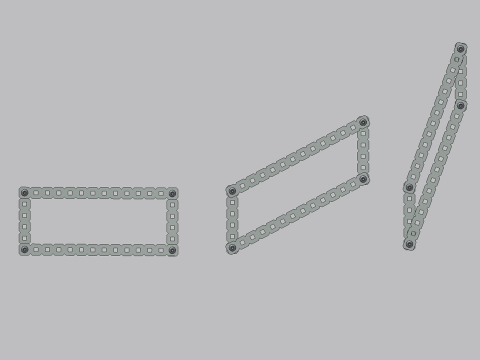
\includegraphics[width=\textwidth,height=5cm,keepaspectratio=true]{Lifts/twoBarCurr}
    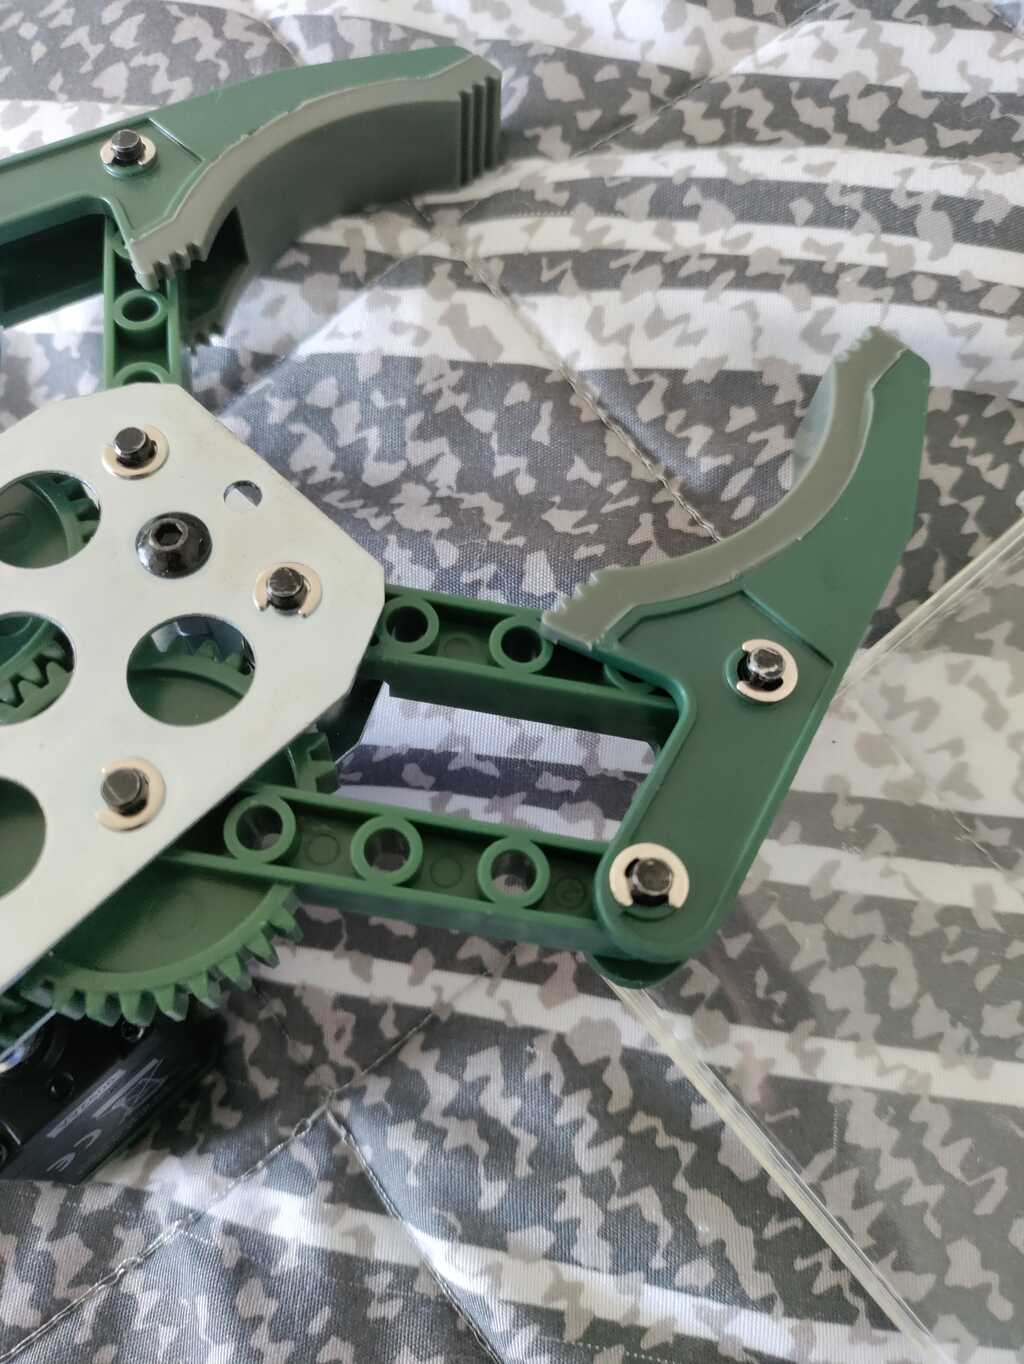
\includegraphics[width=\textwidth,height=5cm,keepaspectratio=true]{Lifts/twobarclaw}
    \caption{
    (Left) Diagram of a four-bar linkage from the VEX curriculum \cite{LinkageCurr}. Notice how the right side of this rectangle stays parallel to the one on the left. (Right) A four-bar linkage found in the vex claw itself!
    }
\end{figure}

\begin{figure}[h]
    \centering
    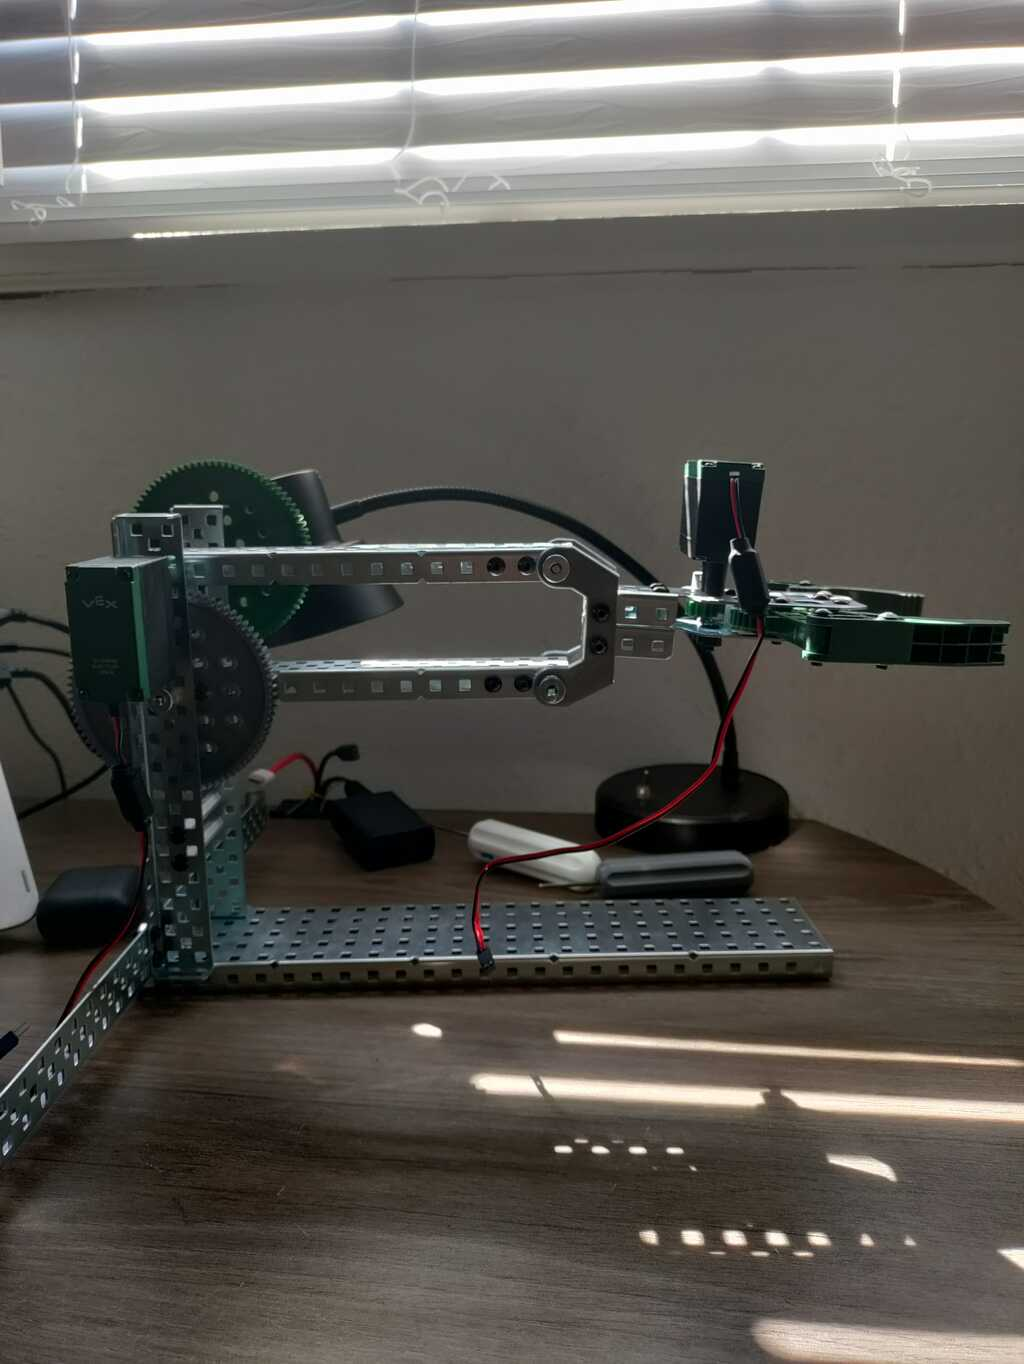
\includegraphics[width=\textwidth,height=5cm,keepaspectratio=true]{Lifts/twoBar1}
    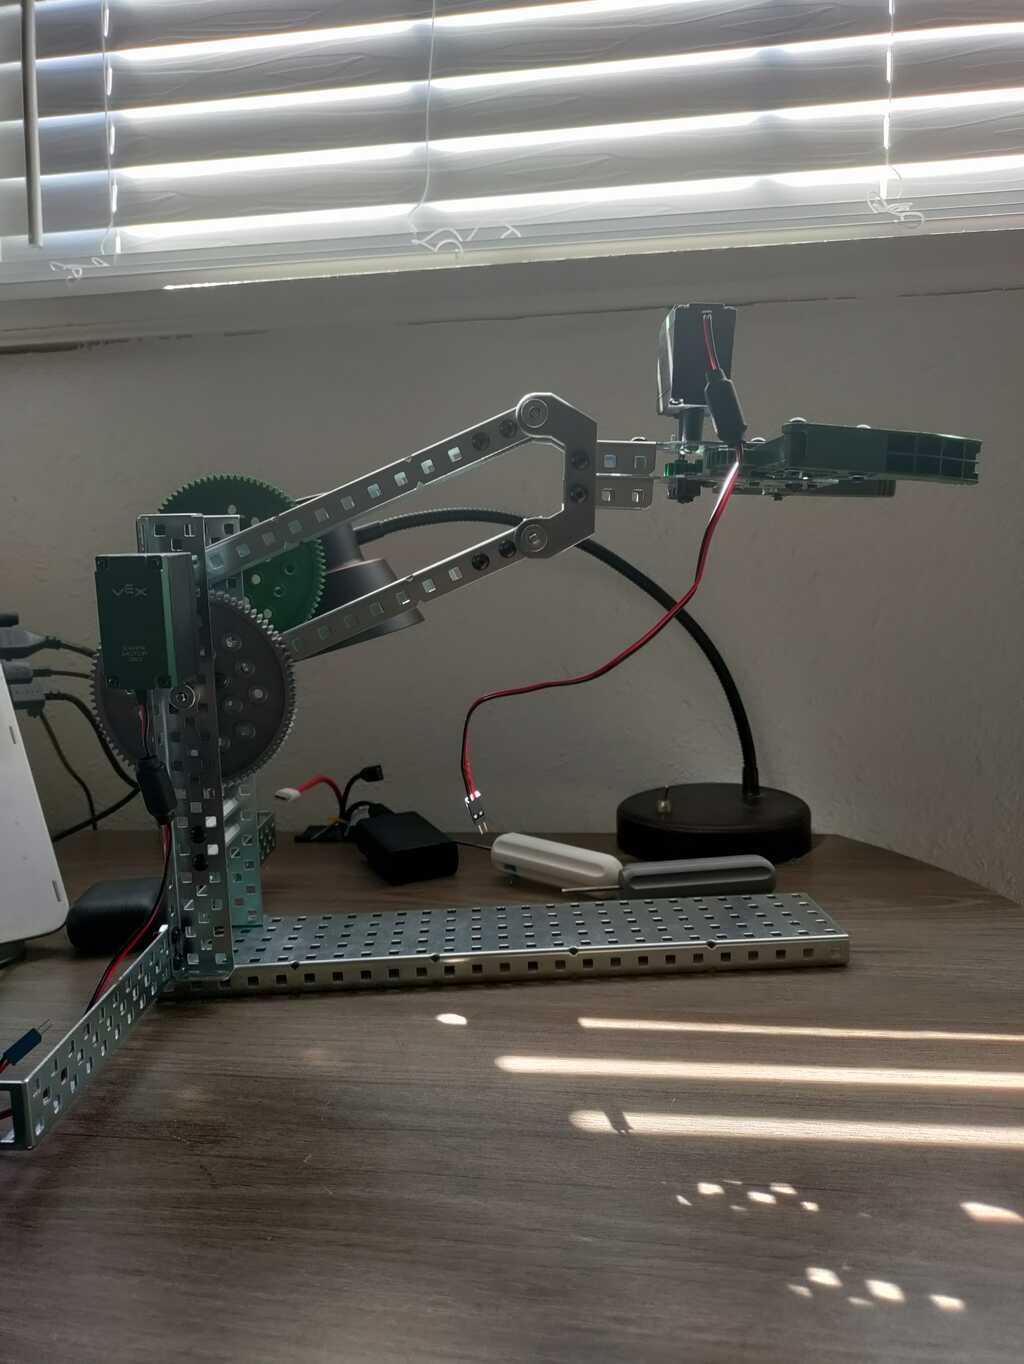
\includegraphics[width=\textwidth,height=5cm,keepaspectratio=true]{Lifts/twoBar2}
    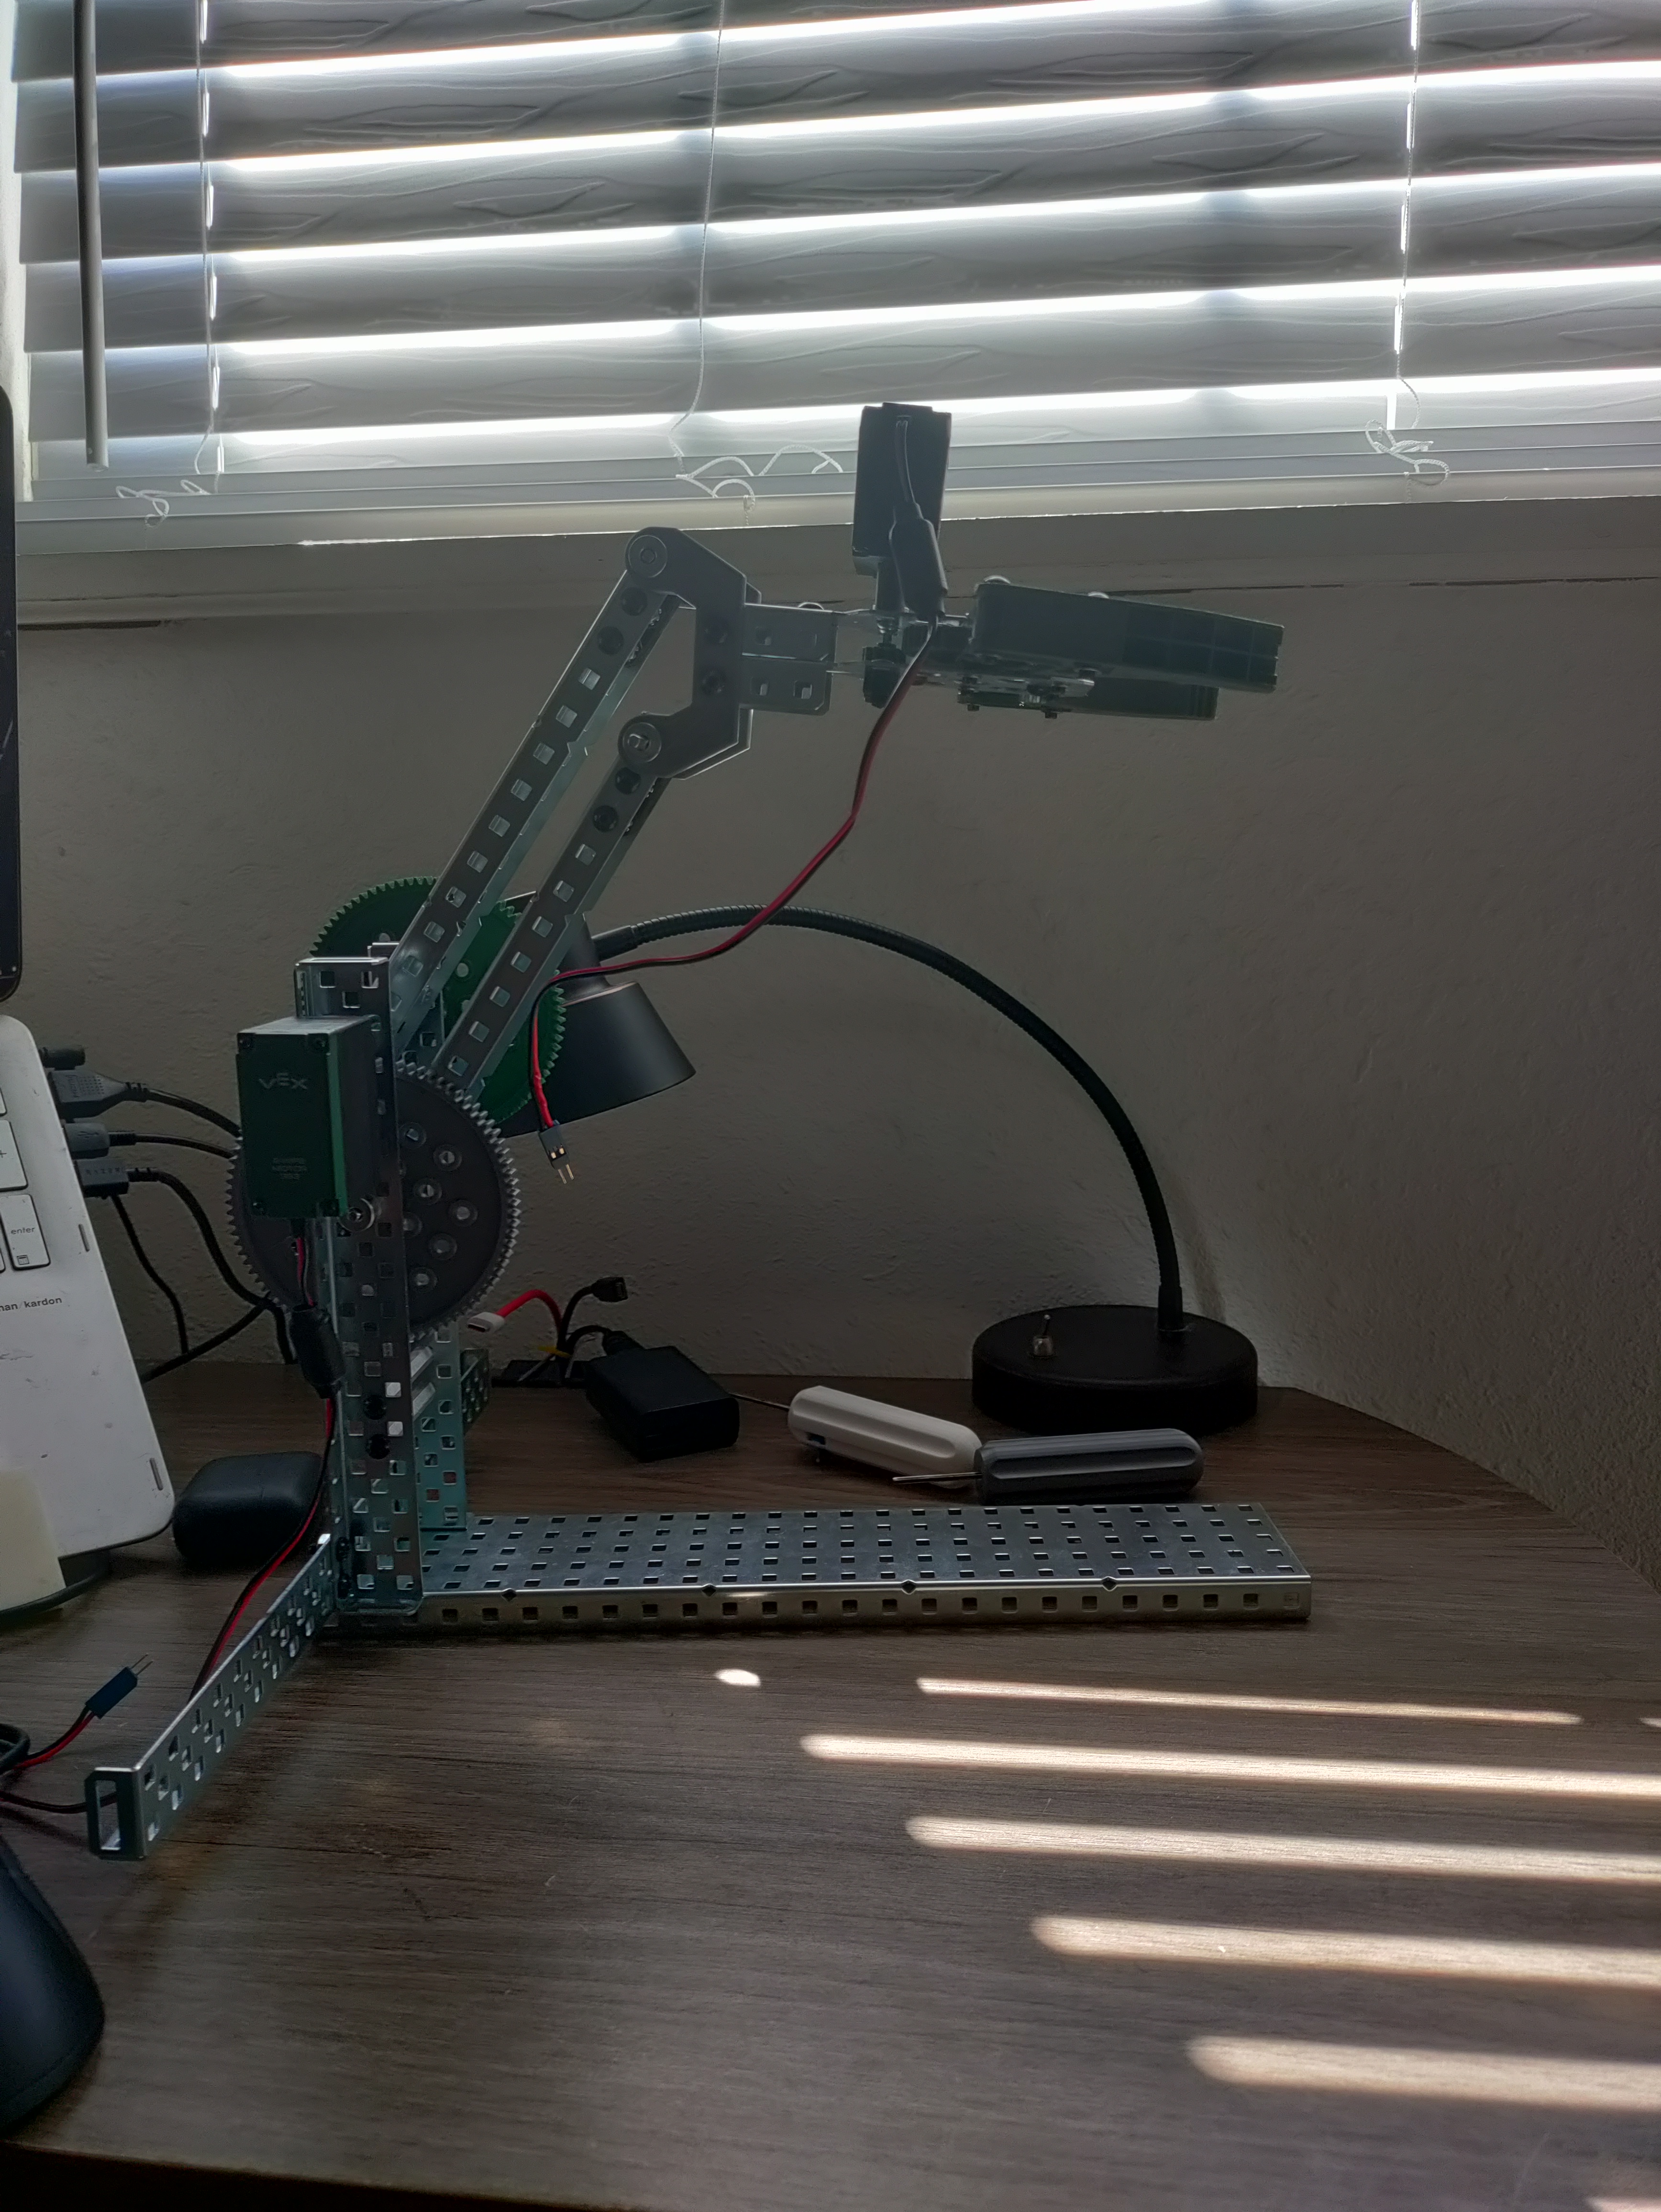
\includegraphics[width=\textwidth,height=5cm,keepaspectratio=true]{Lifts/twoBar3}
    \caption{
    That same four-bar linkage in real life, but the claw assembly is attached to the right side of the rectangle via a special 3D printed part. Notice how the arm stays level to the ground while being at a higher elevation.
    }
\end{figure}

The simplest type of lift is a four-bar lift and is the most intuitive. If four bars are attached to each other to form a rectangle, any rotation in one bar will cause an equal force and rotation to the bar on the the other side. Using this principle, you can use a motor in just the right position so that a claw is parallel to the bar holding up the motor, thus making a self-leveling mechanism useful for stacking objects; This is what all lifts do.

Here are a list of other lifts. While each require more metal and are exponentially harder to create, they are modular, can carry much heavier and bigger objects, and can reach farther.


\begin{figure}[h]
    \centering
    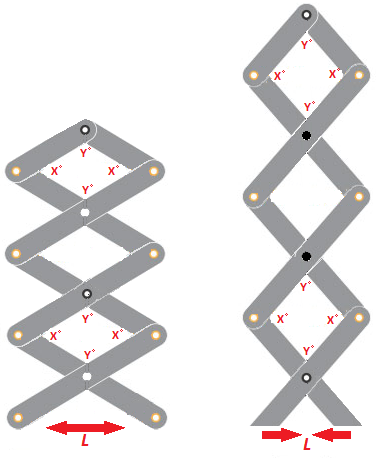
\includegraphics[width=\textwidth,height=4cm,keepaspectratio=true]{Lifts/ScissorDiagram}
    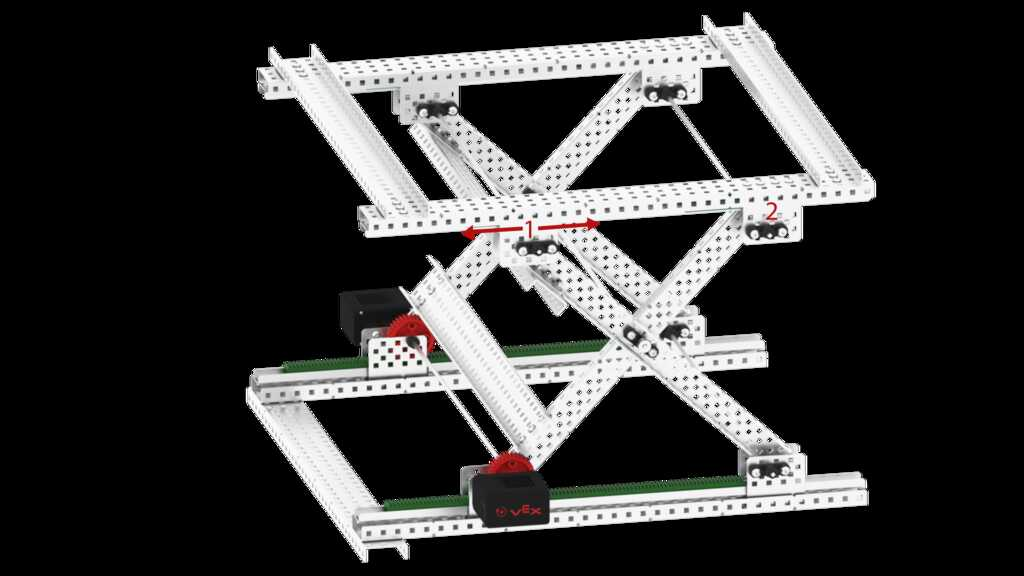
\includegraphics[width=\textwidth,height=4cm,keepaspectratio=true]{Lifts/scissorlift}
    \caption{
    This is a scissor lift, so-called as it requires a scissor-like action to operate. (Left) is the diagram of how a scissor lift extends \cite{ScissorDiagram}, and (Right) is the scissor lift assembly with V5 parts \cite{V5Lifts}. While useful in certain situations, scissor lifts are inefficient, prone to jams, and cannot balance under heavy loads.
    }
\end{figure}


\begin{figure}[h]
    \centering
    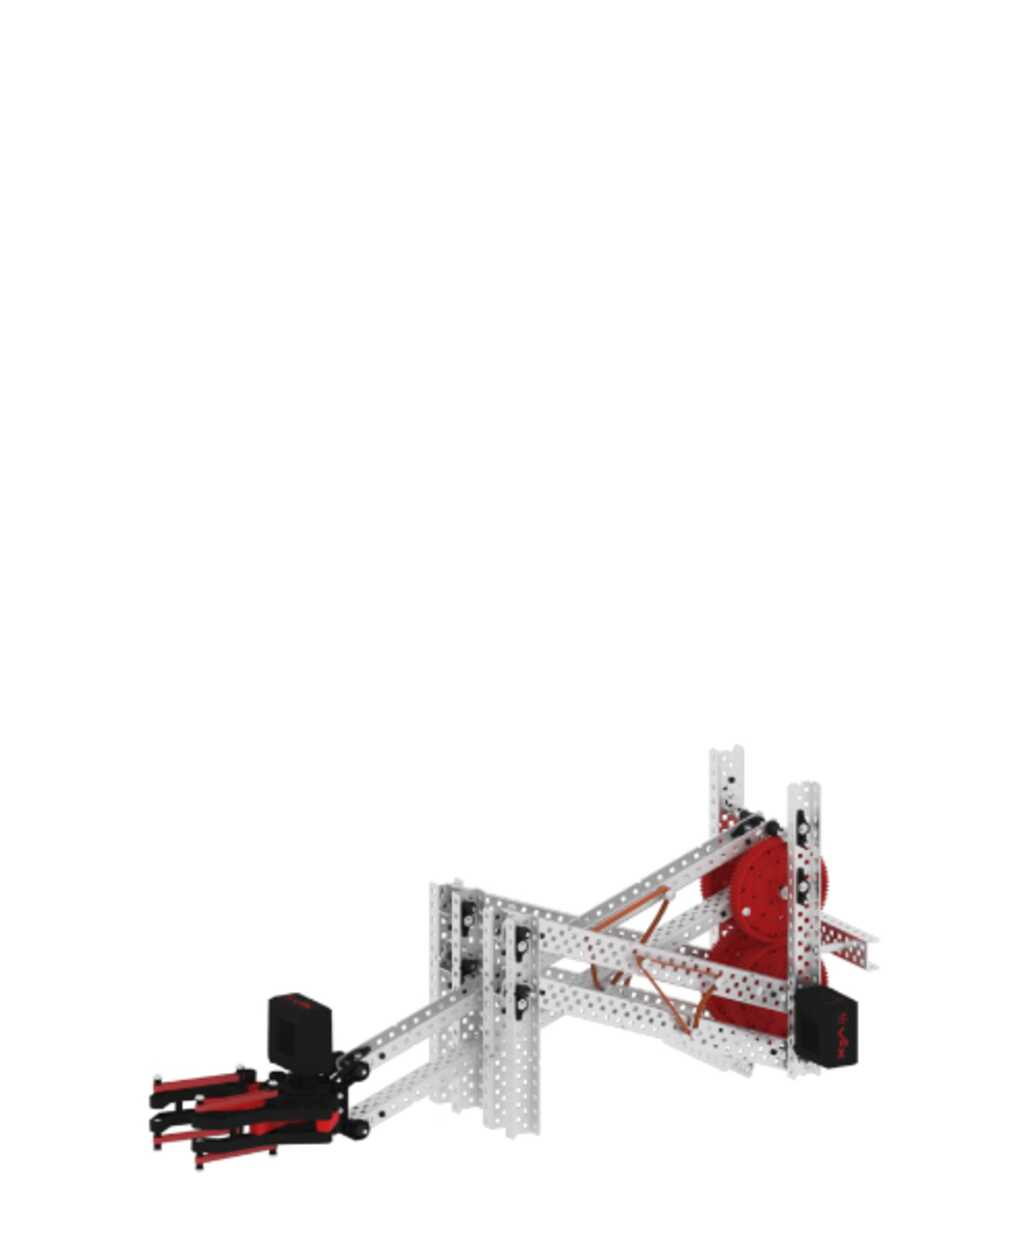
\includegraphics[width=\textwidth,height=4cm,keepaspectratio=true]{Lifts/doublerev1}
    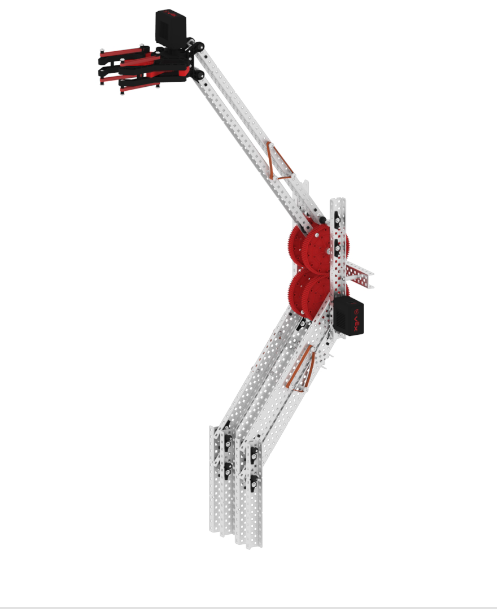
\includegraphics[width=\textwidth,height=4cm,keepaspectratio=true]{Lifts/doublerev2}
    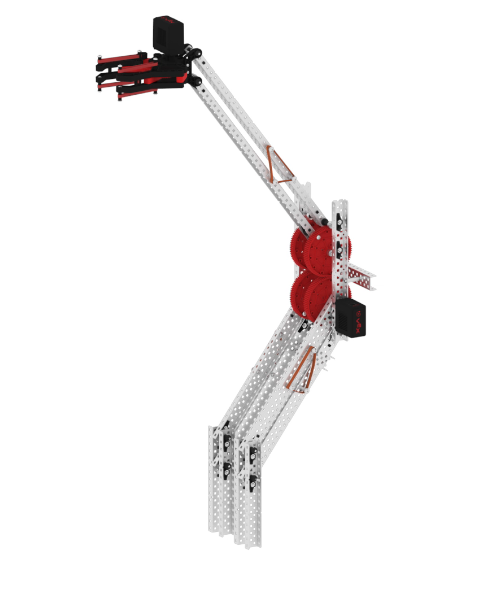
\includegraphics[width=\textwidth,height=4cm,keepaspectratio=true]{Lifts/doublerev3}
    \caption{
    This is a reverse four-bar from the official V5 website \cite{V5Lifts}. Unlike the regular four-bar, this mechanism can \textit{only} move up and does \textit{not} extend out and in of the robot as both four-bars cancel out this movement. This design is commonly seen in professional VEX tournaments as this mechanism does not exert an excessive torque on the robot when fully extended, unlike the regular four-bar. Due to this, a robot with this lift \textit{cannot} tip over with regular usage; It's impossible.
    }
\end{figure}

\begin{figure}[h]
    \centering
    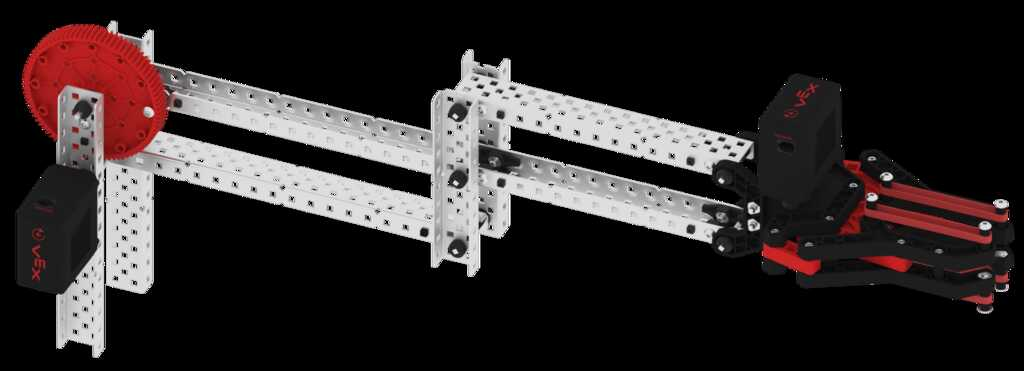
\includegraphics[width=\textwidth,height=3cm,keepaspectratio=true]{Lifts/sixbar}
    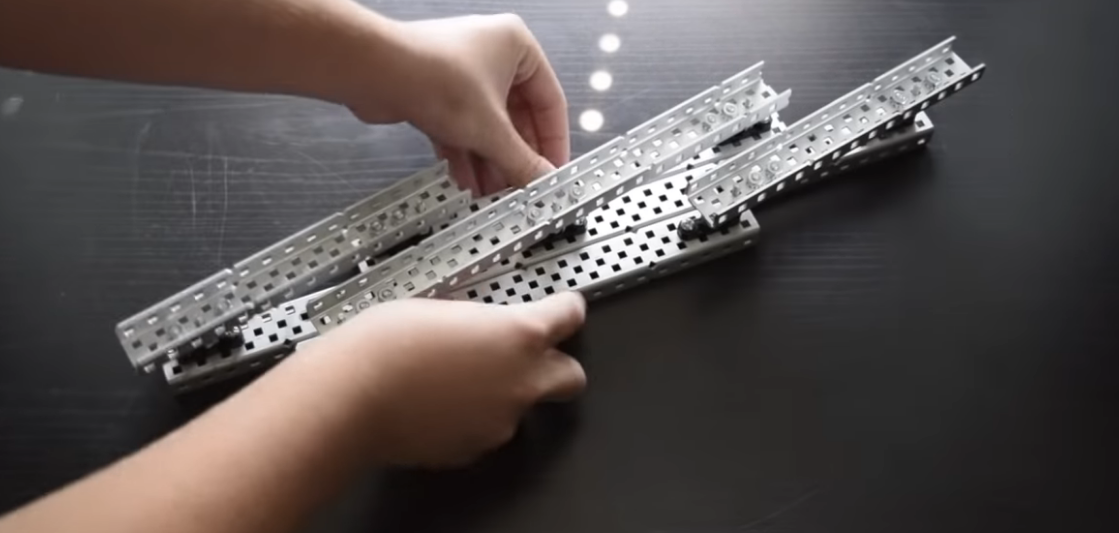
\includegraphics[width=\textwidth,height=3cm,keepaspectratio=true]{Lifts/sixbar1}
    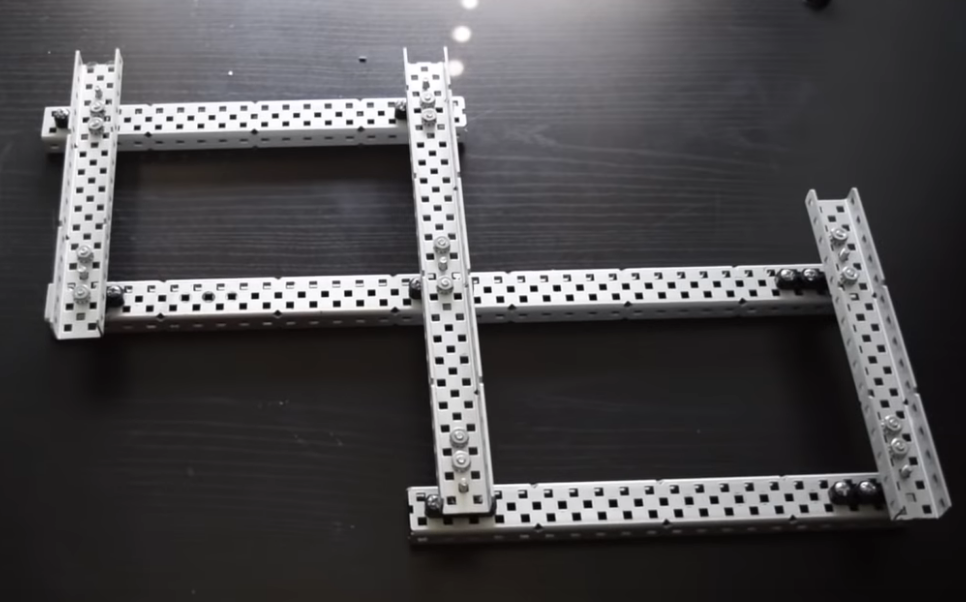
\includegraphics[width=\textwidth,height=3cm,keepaspectratio=true]{Lifts/sixbar2}
    \caption{
    This is a six-bar, which is just a regular lift that extends further than the four bar. (Top) is the assembly using V5 parts \cite{V5Lifts}, and (Middle) and (Bottom) are photos showing how the mechanism still has parallel bars \cite{KeplerLifts}. However, more motors are required to power this mechanism as the torque exerted when at full length is to much for a single 393 motor without rubber bands.
    }
\end{figure}

\begin{figure}[h]
    \centering
    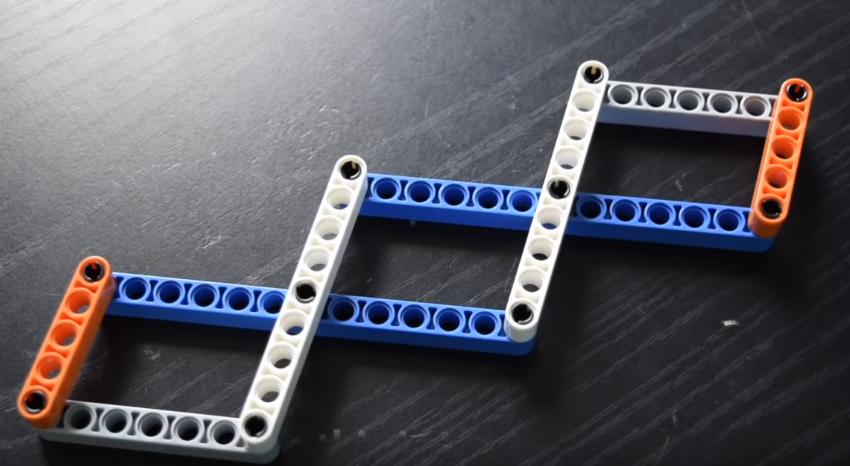
\includegraphics[width=\textwidth,height=4cm,keepaspectratio=true]{Lifts/eightbar1}
    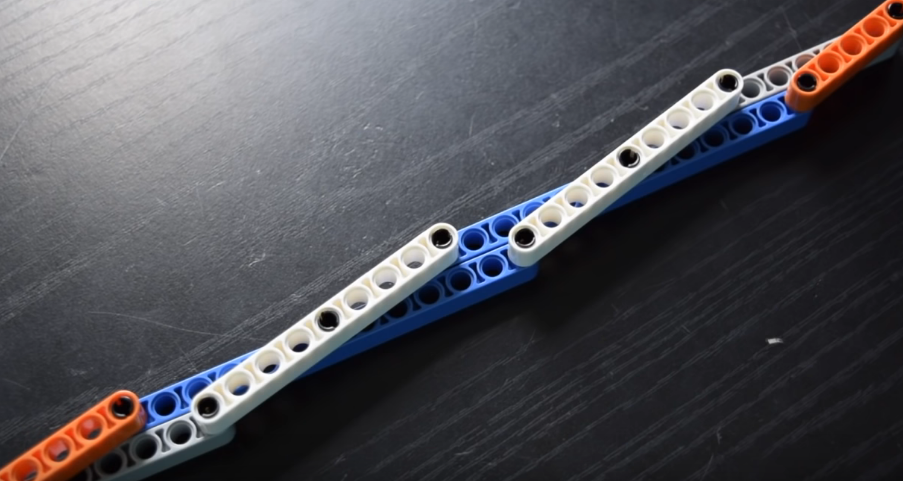
\includegraphics[width=\textwidth,height=4cm,keepaspectratio=true]{Lifts/eightbar2}
    \caption{
    This is an eight-bar, and is simply another extension of the six-bar \cite{KeplerLifts}. In fact, these extensions have no limit given you have a motor powerful enough to handle the torque.
    }
\end{figure}
